\documentclass[12pt]{article}
\usepackage{graphicx}
\usepackage{amsmath}
\usepackage{hyperref}
\usepackage{float}
\usepackage{xcolor}
\usepackage{subcaption}
\usepackage{tikz}
\usepackage{tcolorbox}
\usepackage{algorithm}
\usepackage{algorithmic}
\usepackage{algpseudocode}
\usepackage{amsthm}

\definecolor{darkgreen}{rgb}{0.0, 0.5, 0.0}


\newtheorem{lemma}{Lemma}
\newtheorem{theorem}{Theorem}
\theoremstyle{remark}
\newtheorem*{proof}{Proof}

\begin{document}


\begin{titlepage}
    \begin{center}
        \large    
        \textbf{Bangladesh University of Engineering \& Technology}
            
        \vspace{0.5cm}
        \LARGE
            Computer Science and Engineering
        
        \vspace{1.5cm}
            
        \LARGE
            BYZANTINE GENERALS PROBLEM
        \vspace{1.5cm}  
     \end{center}  
     
\raggedright

\Large
    \textbf{Supervisor}:
    \vspace{0.2cm}\\
\Large
    Abdur Rafi
    \vspace{0.125cm}\\

\raggedleft

\Large
    \textbf{Report written by}:
    \vspace{0.125cm}\\
  \Large
    2105123-Shatabdi Dutta Chowdhury
    \vspace{0.125cm}\\
    2105124-Shadman Abid
    \vspace{0.125cm}\\
    2105129-Sarowar Alam Roki

    \vspace{5cm}
        \begin{center}
            \large
            \textbf{Date:} \today
        \end{center}
    
\end{titlepage}

\tableofcontents
\newpage

\begin{center}
    \LARGE \textbf{Byzantine Generals Problem}
\end{center}

\vspace{1 cm}

\begin{abstract}
In a distributed computer system, some components may behave unpredictably or maliciously, sending conflicting information that disrupts overall operations. This challenge can be likened to achieving agreement among system nodes communicating through unreliable channels, even when some act dishonestly. The key problem is developing a protocol that ensures consensus among trustworthy components, regardless of disruptions. Research shows that consensus is possible with basic communication methods if the number of faulty components remains below a certain threshold. With secure mechanisms like cryptographic authentication, consensus can be achieved even with an arbitrary number of faulty components. These principles are essential for designing fault-tolerant systems capable of reliable operation despite failures or adversarial behavior.
\end{abstract}

\section*{\centering Introduction}
\addcontentsline{toc}{section}{Introduction}

Reliable computer systems must be designed to withstand failures, even when some components behave erratically or maliciously. A critical challenge arises when faulty components send conflicting information to different parts of the system, undermining coordination and decision-making. This problem is often abstracted as a distributed agreement challenge, famously referred to as the Byzantine Generals Problem.

\textit{In this analogy, several divisions of an army are encamped around a city, each led by a general. These generals must coordinate a unified strategy—whether to attack or retreat—using only messengers for communication. However, some generals may act as traitors, sending contradictory messages to sow confusion and disrupt the consensus. The loyal generals must devise a strategy to ensure that all their divisions act in unison, regardless of any attempts by traitors to undermine the plan.}

This vivid scenario encapsulates the essence of challenges faced in distributed systems, where achieving agreement in the presence of faults or malicious actors is critical. Achieving consensus requires protocols that ensure all loyal participants agree on a plan, while remaining robust against interference. This paper examines this abstract problem, providing strategies to ensure agreement in adversarial settings and discussing their application in fault-tolerant system design.

\section*{\centering Problem Formulation}
\addcontentsline{toc}{section}{Problem Formulation}
To address the Byzantine Generals Problem, we model the system as a group of generals coordinating through unreliable channels. Each general observes external conditions and communicates their observations to others, forming a collective decision. Two critical conditions must be met:\\

\textbf{Consistency (C1)}: All loyal generals must agree on the same course of action, regardless of any traitorous interference.

\textbf{Correctness (C2)}: If the commanding general is loyal, all loyal generals must follow the order they issue.\\
These conditions ensure that malicious actions cannot disrupt agreement or lead loyal participants to an undesirable decision. However, satisfying these conditions is complex because traitorous participants can send contradictory information, potentially misleading different groups of loyal generals.
\\
\\
To better understand the parallels between distributed systems and the Byzantine Generals Problem, consider the example illustrated in figure \ref{fig:byzantine_faults}. In distributed systems, faults may arise from components sending conflicting or false data, analogous to traitorous generals issuing misleading commands. By designing robust protocols, both systems ensure consensus among loyal participants despite adversarial interference.

\begin{figure}[H] \centering 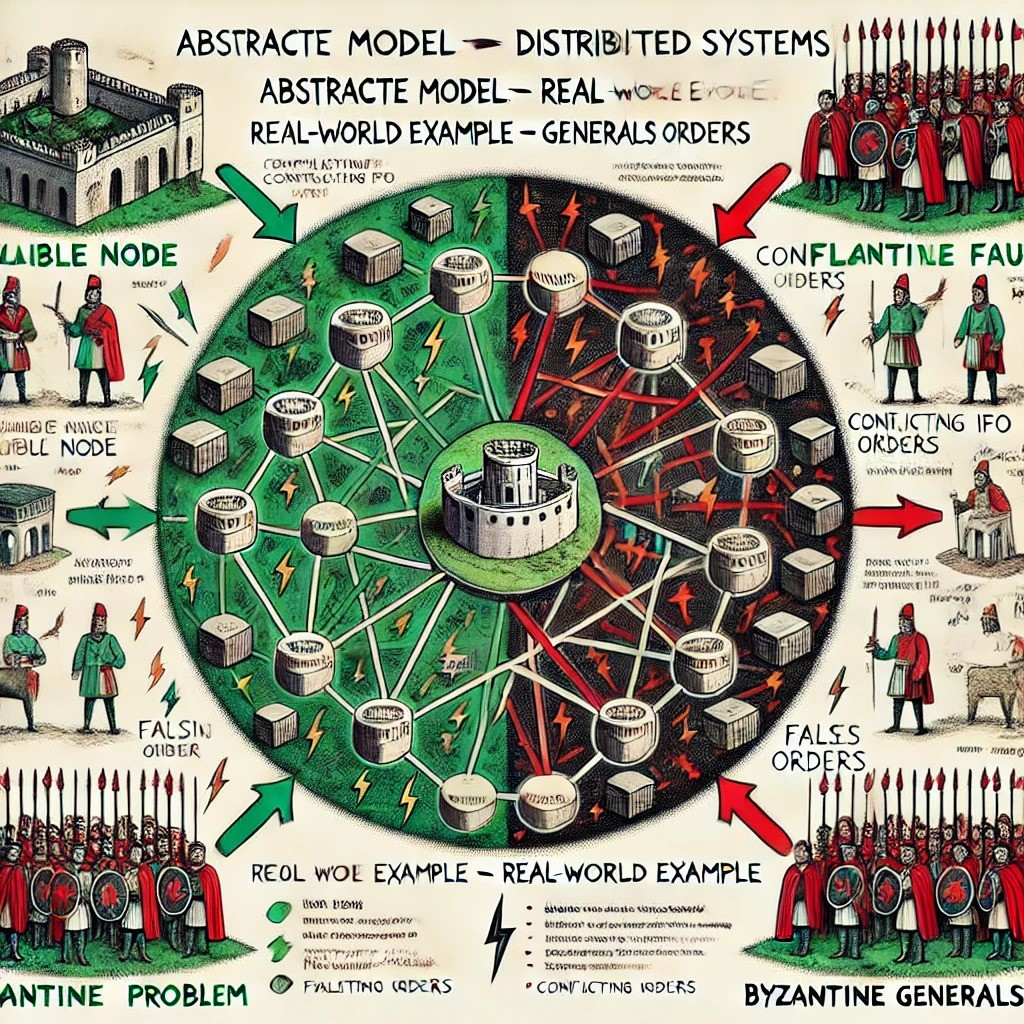
\includegraphics[width=0.9\textwidth]{images/Byz1.jpg}
\caption{Byzantine Faults in Distributed Systems and the Generals Analogy. Reliable participants must achieve consensus despite malicious actors sending conflicting information.} \label{fig:byzantine_faults} \end{figure}

To ensure \textcolor{darkgreen}{consistency and correctness}, every general must use the same method for processing and combining information. For instance, if the decision involves a binary choice, a majority vote can help achieve consensus, provided the number of traitorous participants is limited. The problem becomes ensuring that every loyal participant receives consistent and accurate information, even if some generals deliberately send false or conflicting data. This requires robust communication protocols and mechanisms to authenticate messages, minimizing the influence of malicious actors and preserving the integrity of the decision-making process.

\section*{\centering Impossibility Results}
\addcontentsline{toc}{section}{Impossibility Results}

The Byzantine Generals Problem may seem deceptively simple, but its complexity lies in the surprising fact that if the generals communicate using only oral messages, no solution can work unless more than two-thirds of the generals are loyal. For instance, with only three generals, no solution can tolerate even a single traitor. An \textbf{\emph{oral message}} is one whose contents are entirely controlled by the sender, allowing a traitorous sender to transmit any message. Such a message is analogous to the type of communication typically used by computers.

\vspace{2cm}

\begin{figure}[h!]
    \centering
    \begin{subfigure}[b]{0.45\textwidth}
        \centering
        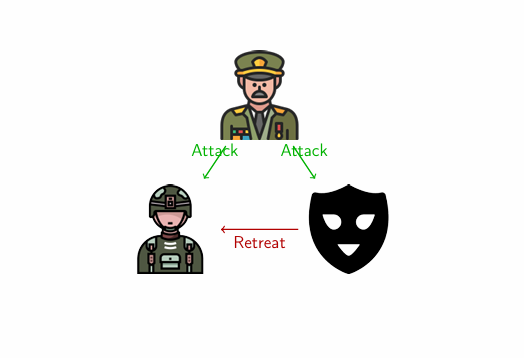
\includegraphics[width=\textwidth]{images/scene1.png}
        \caption{Case 1}
        \label{fig:image1}
    \end{subfigure}
    \hspace{0.5cm}  
    \begin{subfigure}[b]{0.45\textwidth}
        \centering
        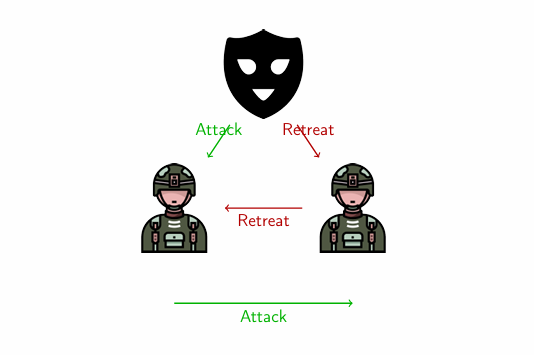
\includegraphics[width=\textwidth]{images/scene2.png}
        \caption{Case 2}
        \label{fig:image2}
    \end{subfigure}
    
    \caption{Two Scenerios}
    \label{fig:sidebyside}
\end{figure}

\vspace{2cm}

To illustrate this, consider two scenarios:
\begin{enumerate}
    \item In the first scenario, the commander is loyal and sends an ``attack'' order, but Lieutenant 2 is a traitor who tells Lieutenant 1 that the commander sent a ``retreat'' order.
    \item In the second scenario, the commander is a traitor who sends an ``attack'' order to Lieutenant 1 and a ``retreat'' order to Lieutenant 2.
\end{enumerate}

In both cases, Lieutenant 1 cannot distinguish between the two scenarios because the traitor can lie consistently. Thus, if Lieutenant 1 obeys the ``attack'' order in the first scenario, he must also obey it in the second scenario. Similarly, a similar argument applies to Lieutenant 2. This situation violates the integrity conditions:

\begin{tcolorbox}[colframe=green!80!black, colback=green!10!white, coltitle=black, title=Integrity Conditions]
\begin{itemize}
    \item \textbf{IC1}: All loyal generals obey the same order.
    \item \textbf{IC2}: If the commander is loyal, then every loyal lieutenant obeys the order sent by the commander.
\end{itemize}
\end{tcolorbox}

Hence, no solution exists for three generals with one traitor. This argument may appear plausible but lacks rigorous proof. For a formal proof, refer to \cite{lamport1982byzantine}. Using this result, it is proven that no solution with fewer than $3m + 1$ generals can handle $m$ traitors.
\renewcommand\thesubsection{\arabic{subsection}}
\subsection{Mathematical Proof}

To avoid confusion, we differentiate between the two algorithms by naming the generals of the assumed solution \emph{Albanian generals} and those of the constructed solution \emph{Byzantine generals}. Assuming a solution exists for $3m$ or fewer Albanian generals to tolerate $m$ traitors, we construct a solution for three Byzantine generals to handle a single traitor.

Each Byzantine general simulates $\approx m$ Albanian generals. Specifically:

\[
\begin{aligned}
\text{\textbf{Byzantine Commander:}} & \quad m-1 \text{ Albanian Lieutenants + Albanian Commander,} \\
\text{\textbf{Byzantine Lieutenants:}} & \quad \text{At most } m \text{ Albanian Lieutenants each.}
\end{aligned}
\]

Since at most one Byzantine general is a traitor, only $m$ Albanian generals can be traitors. By satisfying IC1 and IC2 for the Albanian generals, the corresponding conditions hold for the Byzantine generals. Thus, a contradiction is reached.

\subsection{Approximate Agreement}

Some may argue that exact agreement is the source of difficulty in the Byzantine Generals Problem. However, even achieving approximate agreement is equally challenging. For approximate agreement, the following modified conditions are required:

\begin{tcolorbox}[colframe=green!80!black, colback=green!10!white, coltitle=black, title=Modified Conditions]
\begin{itemize}
    \item \textbf{IC1'}: All loyal lieutenants attack within 10 minutes of one another.
    \item \textbf{IC2'}: If the commander is loyal, then all loyal lieutenants attack within 10 minutes of the commanded time.
\end{itemize}
\end{tcolorbox}

Using a similar approach, it can be shown that approximate agreement for three generals with one traitor is also impossible. Suppose the commander sends an attack at $1:00$ and a retreat at $2:00$. Each lieutenant executes the following:
\begin{enumerate}
    \item If the received time is:
    \begin{itemize}
        \item $\leq 1:10$, then attack.
        \item $\geq 1:50$, then retreat.
        \item Otherwise, defer the decision.
    \end{itemize}
    \item Ask the other lieutenant's decision. If decided, follow their decision; otherwise, retreat.
\end{enumerate}

By contradiction, this approach also constructs a three-general solution for the original Byzantine Generals Problem, which is impossible. Hence, no solution exists for fewer than $3m + 1$ generals to handle $m$ traitors.

The impossibility of solving the Byzantine Generals Problem, even approximately, highlights the critical role of loyalty thresholds in achieving consensus. The mathematical insights presented here serve as the foundation for future research on fault-tolerant algorithms.



\section*{\centering Solutions}
\addcontentsline{toc}{section}{Solutions}
\subsection*{\textbf{Oral Messages}}
\addcontentsline{toc}{subsection}{Oral Messages}

We aim to solve the Byzantine Generals Problem using oral messages. Let us define an oral message system with the following assumptions:
\begin{itemize}
    \item \textbf{A1}: Every message that is sent is delivered correctly.
    \item \textbf{A2}: The receiver of a message knows who sent it.
    \item \textbf{A3}: The absence of a message can be detected.
\end{itemize}

Let us describe the algorithm \( OM(m) \), for \( m \geq 0 \), to solve the problem with at most \( m \) traitors. We assume the existence of a function \texttt{majority} that returns the majority value from a list, or RETREAT if no majority exists.


\subsubsection*{Algorithm OM(0)}
\addcontentsline{toc}{subsubsection}{Algorithm $OM(0)$}
\begin{algorithm}
\caption{OM(0)}
\begin{algorithmic}[1]
\State The commander sends his value \( v \) to every lieutenant.
\For{each lieutenant \( i \)}
    \If{Lieutenant \( i \) receives no value}
        \State Let \( v_i = \text{RETREAT} \)
    \Else
        \State Let \( v_i \) be the value received from the commander.
    \EndIf
\EndFor
\State Each lieutenant uses the received value \( v_i \), or RETREAT if no value is received.
\end{algorithmic}
\end{algorithm}


\subsubsection*{Algorithm OM(m) for \( m > 0 \)}
\addcontentsline{toc}{subsubsection}{Algorithm $OM(m)$}
\begin{algorithm}[H]
\caption{OM(m)}
\begin{algorithmic}[1]
\State The commander sends his value \( v \) to every lieutenant.
\For{each lieutenant \( i \)}
    \State Let \( v_i \) be the value received from the commander, or RETREAT if no value is received.
    \State Lieutenant \( i \) invokes Algorithm \( OM(m-1) \) with the value \( v_i \) and sends it to every other lieutenant.
\EndFor
\For{each lieutenant \( i \), and each lieutenant \( j \neq i \)}
    \State Let \( v_j \) be the value received by Lieutenant \( i \) from Lieutenant \( j \).
    \If{Lieutenant \( i \) receives no message from Lieutenant \( j \)}
        \State Let \( v_j = \text{RETREAT} \)
    \EndIf
    \State Lieutenant \( i \) computes the majority value \( v_i=\text{majority}(v_1, v_2, \dots, v_{n-1}) \)
\EndFor
\end{algorithmic}
\end{algorithm}



\begin{lemma}
  For any \( m \) and \( k \), Algorithm \( OM(m) \) satisfies IC2 if there are more than \( 2k + m \) generals and at most \( k \) traitors.
\end{lemma}

\subsubsection*{Proof of Lemma 1}
\begin{proof}
\begin{align*}
    \text{Step 1:} \quad & \text{The commander sends a value } v \text{ to all } n-1 \text{ lieutenants.} \\
\text{Step 2:} \quad & \text{Each lieutenant applies Algorithm } OM(m-1) \text{ to all other generals.} \\
\text{Step 3:} \quad & \text{By the induction hypothesis, each lieutenant gets } v_j = v \text{ for each loyal lieutenant.} \\
\text{Step 4:} \quad & \text{Since there are at most } k \text{ traitors, a majority of the values are loyal.} \\
\text{Step 5:} \quad & \text{Thus, each loyal lieutenant computes the majority value } v = \text{majority}(v_1, v_2, \dots, v_{n-1}).
\end{align*}
\end{proof}



\subsection*{Correctness of Algorithm OM(m)}

\begin{theorem}
  Algorithm \( OM(m) \) satisfies conditions IC1 and IC2 if there are more than \( 3m \) generals and at most \( m \) traitors.   
\end{theorem}


\subsubsection*{Proof of Theorem 1}

\begin{proof}
   We prove the theorem by induction on \( m \).

\textbf{Base Case:} When \( m = 0 \), the commander sends the value \( v \) to all lieutenants. Since no traitors exist, all lieutenants get the same value \( v \). Thus, IC1 and IC2 are satisfied.

\textbf{Inductive Step:} Assume that the theorem holds for \( m-1 \). Now, consider \( m > 0 \). If the commander is loyal, then by Lemma 1, OM(m) satisfies IC2. IC1 follows from IC2 for loyal commanders.

If the commander is a traitor, at most \( m-1 \) lieutenants are traitors. Since there are more than \( 3m \) generals, there are more than \( 3m-1 \) lieutenants, and \( 3m-1 > 3(m-1) \). Thus, by the induction hypothesis, OM(m-1) satisfies IC1 and IC2 for each lieutenant. Hence, the loyal lieutenants compute the same majority value in step 3, satisfying IC1. 
\end{proof}



\subsection*{\textbf{Signed Messages}}
\addcontentsline{toc}{subsection}{Signed Messages}
Signed messages introduce digital signatures to authenticate communication, ensuring that malicious actors cannot forge orders. This method significantly improves fault tolerance.

\section*{\centering Applications}
\addcontentsline{toc}{section}{Applications}
\renewcommand\thesubsection{A.\arabic{subsection}}
\subsection{Blockchain and Cryptocurrencies}
Byzantine Fault Tolerance (BFT) algorithms ensure consensus in decentralized systems, such as Bitcoin and Ethereum, even in the presence of malicious nodes.

\subsection{Distributed Databases}
Ensuring consistent data across nodes in distributed databases often relies on BFT principles to handle faults and maintain reliability.

\section*{\centering Conclusion}
\addcontentsline{toc}{section}{Conclusion}
The Byzantine Generals Problem is a cornerstone of reliability in distributed systems. It enables consensus, scalability, and resilience, making it essential for modern decentralized technologies like blockchain.


\newpage
\bibliographystyle{plain}
\bibliography{ref}

\begin{quote}
"By leveraging BFT protocols, we build systems that stand strong amidst failures."
\end{quote}

\end{document}
